\hypertarget{rt__init_8c}{
\section{rt\_\-init.c File Reference}
\label{rt__init_8c}\index{rt_init.c@{rt\_\-init.c}}
}


\subsection{Detailed Description}
\begin{Desc}
\item[For internal use only.]
This file contains the implementation of the \hyperlink{group__dbprim__rbtree_ga6}{rt\_\-init()} function, used to dynamically initialize a red-black tree.\end{Desc}


Definition in file \hyperlink{rt__init_8c-source}{rt\_\-init.c}.

{\tt \#include \char`\"{}dbprim.h\char`\"{}}\par
{\tt \#include \char`\"{}dbprim\_\-int.h\char`\"{}}\par


Include dependency graph for rt\_\-init.c:\begin{figure}[H]
\begin{center}
\leavevmode
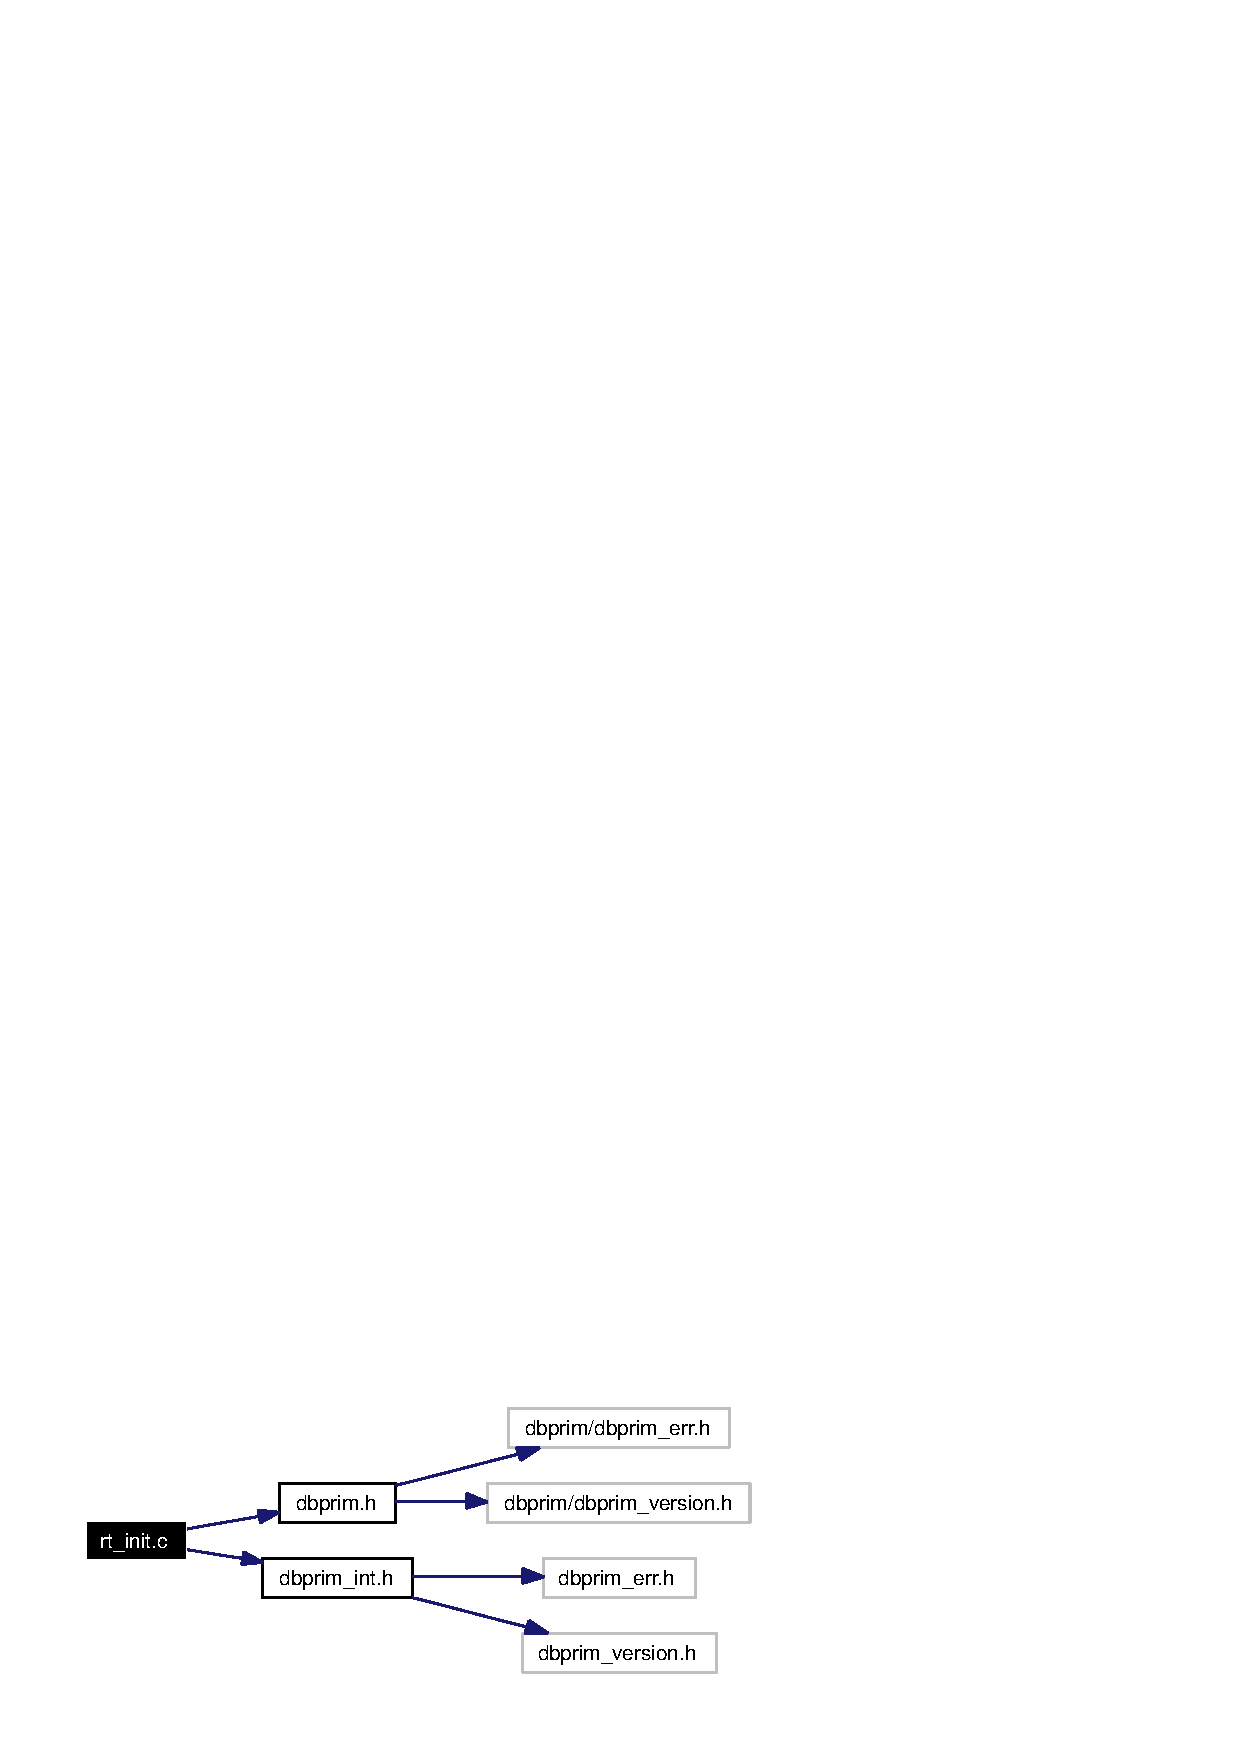
\includegraphics[width=182pt]{rt__init_8c__incl}
\end{center}
\end{figure}
\subsection*{Functions}
\begin{CompactItemize}
\item 
unsigned long \hyperlink{group__dbprim__rbtree_ga6}{rt\_\-init} (\hyperlink{struct__rb__tree__s}{rb\_\-tree\_\-t} $\ast$tree, \hyperlink{group__dbprim__rbtree_ga3}{rb\_\-comp\_\-t} comp, void $\ast$extra)
\begin{CompactList}\small\item\em Dynamically initialize a red-black tree. \item\end{CompactList}\end{CompactItemize}
